\header{
    \headtitle{Tous les chemins mènent au rhum} \label{tous-les-chemins-menent-au-rhum}
    %
    \insertComment{Paroles et musique de Xavier Pétermann pour Corrigan Fest.}{}
}

\enluminure{4}{\href{https://www.youtube.com/watch?v=CvPwZhXTXUo}{D}}{epuis} que je suis tout petit ma mère m'a répété
\\Petit fais attention, tu n'es pas très futé
\\Ton père était comme toi, il est mort à la guerre
\\En chantant des chansons et en buvant de la bière
\\À tous ceux qui m'accusent de faire pleurer Maman
\\Parce que j'ai pris la route le jour de mes seize ans
\\À ceux-là je réponds que je pourrais faire pire
\\Je pourrais regretter et penser à revenir
\\\\\textbf{Refrain :}
\\Lève ton verre mon ami, le jour n'est pas fini
\\Le soleil brille encore sur nos sombres remords
\\Et partout où qu'on aille sur cette terre des Hommes
\\Il n'y a qu'une vérité : tous les chemins mènent au rhum
\\\\Une nuit dans une ruelle, j'ai croisé un vieillard
\\Des cornes ornaient son front et ses yeux étaient noirs
\\Il m'a montré un pacte que je devais signer
\\Je pris la plume et sans vouloir, renversai l'encrier
\\À tous ceux qui m'accusent d'avoir mon âme au diable vendue
\\Quand il a vu qui j'étais, même lui n'en a pas voulu
\\Il m'a dit qu'il n'avait que faire de l'âme des crétins
\\Il m'a dit garde ton âme, pousse tes fesses et reprends ton chemin
\\\\Par un matin d'avril au détour d'un chemin
\\J'ai croisé une fille mi-princesse mi-putain
\\Elle voulut m'embrasser et faire de moi un roi
\\Je ne pus refuser, c'était ma première fois
\\À tous ceux qui m'accusent d'avoir cédé à la tentation
\\C'est que j'aurais bien voulu mais je n'en eus point l'occasion
\\Car dès que j'eus les yeux fermés dans un délicieux soupir
\\Elle m'assomma, me prit mes biens et me laissa mourir
\\\\Aujourd'hui je suis là au paradis des cons
\\Du haut de mon nuage, je chante cette chanson
\\Je bouffe des goélands et je bois de la bière
\\Je pisse pour faire la pluie et je rote pour le tonnerre
\\Aujourd'hui je suis là au paradis des imbéciles
\\Quand je regarde en bas, des fois, je trouve ça difficile
\\Alors je me saoule la gueule et je dégringole de mon nuage
\\Si j'étais aussi gros que con ça ferait un vrai carnage
\bigskip
\bigskip
\begin{center}
\centering
    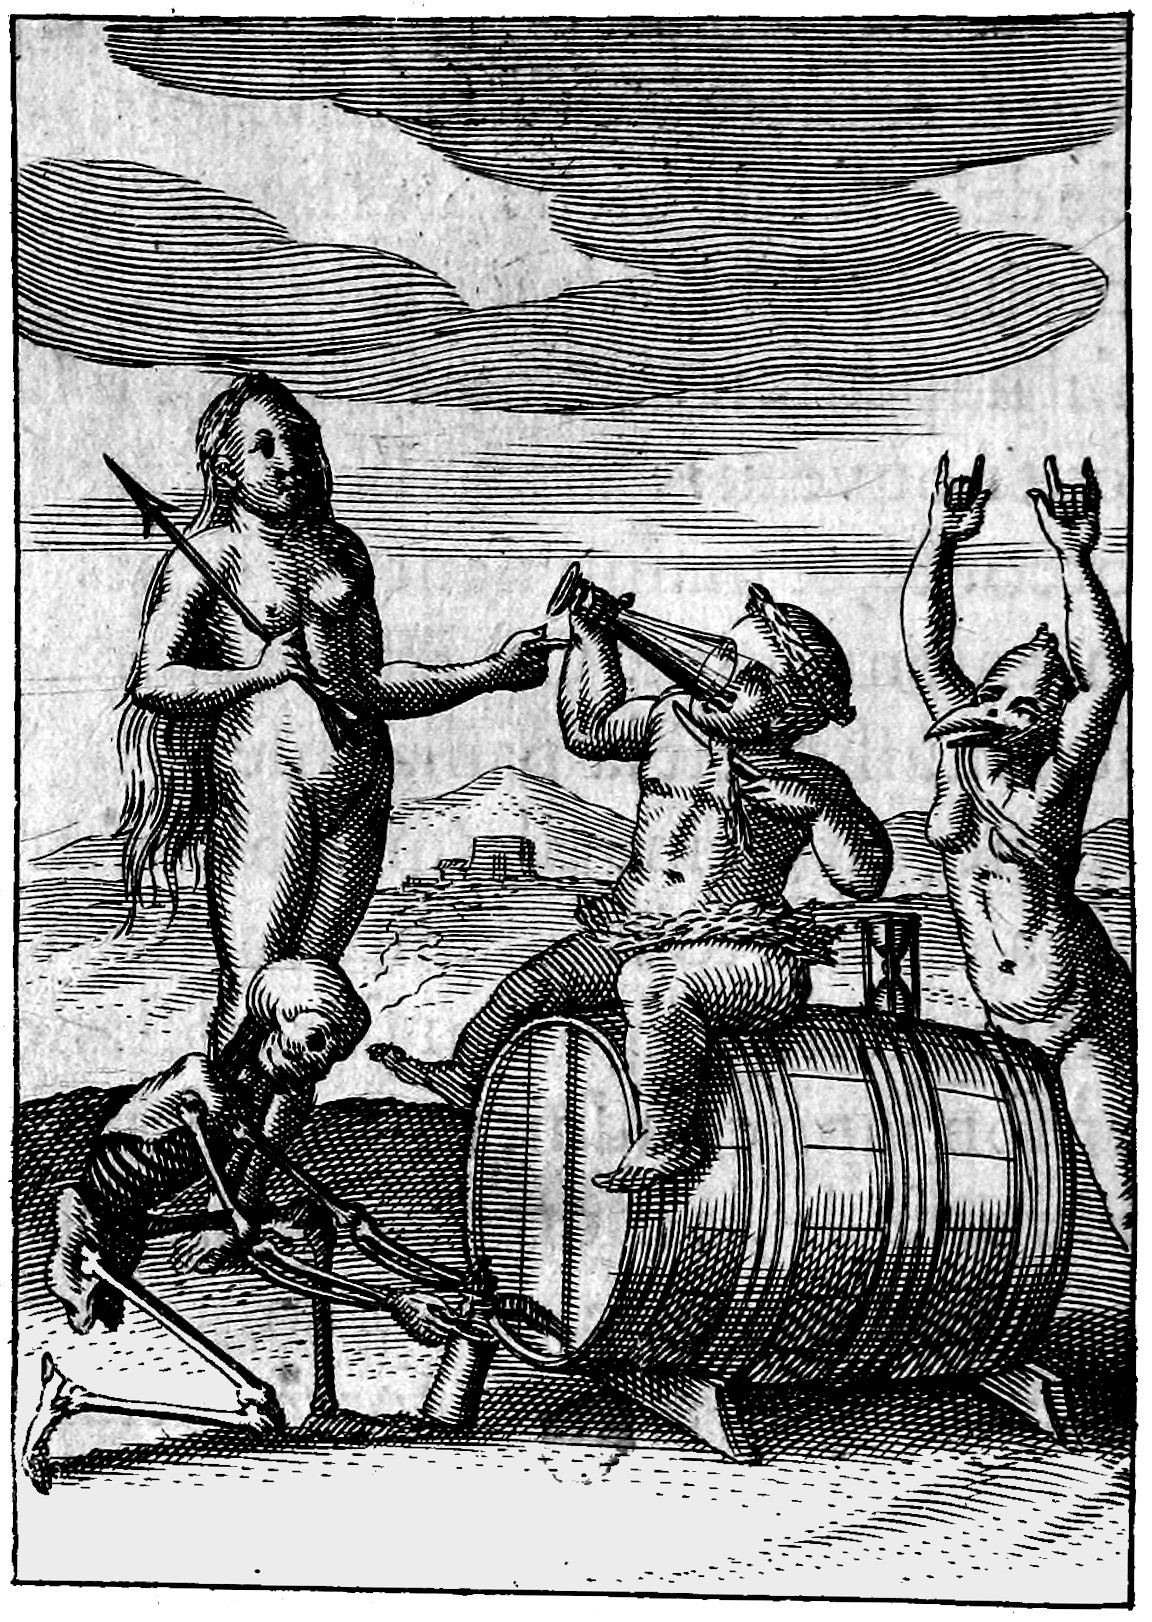
\includegraphics[width=0.8\textwidth]{images/brev1.png}
 \end{center}
\breakpage